\documentclass[tikz,border=2pt]{standalone}
\usepackage{amsmath,amssymb}
\usepackage{tikz}
\usetikzlibrary{arrows.meta,decorations.pathreplacing}

\begin{document}
% S=(0,1): every number >= 1 is an upper bound; the least of them, sup S = 1, is not in S.
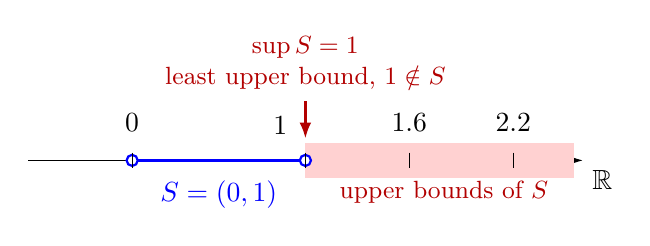
\begin{tikzpicture}[x=2.2cm]
	\draw[-{Latex[length=2.5mm]}] (-0.6,0) -- (2.6,0) node[below right] {$\mathbb{R}$};
	\fill[red!18] (1,-0.22) rectangle (2.55,0.22);
	\draw[very thick, blue] (0,0) -- (1,0);
	\draw[blue, thick, fill=white] (0,0) circle (2pt);
	\draw[blue, thick, fill=white] (1,0) circle (2pt);
	\node[blue, below=4pt] at (0.5,0) {$S=(0,1)$};
	\foreach \x/\l in {0/$0$, 1.6/$1.6$, 2.2/$2.2$} {\draw (\x,0.1) -- (\x,-0.1); \node[above=4pt] at (\x,0.1) {\l};}
	\draw (1,0.1) -- (1,-0.1);
	\node[above left=3pt] at (1,0.1) {$1$};
	\node[red!70!black, below=4pt, font=\small] at (1.8,0) {upper bounds of $S$};
	\draw[-{Latex[length=2mm]}, red!70!black, thick] (1,0.75) -- (1,0.28);
	\node[red!70!black, above, font=\small, align=center] at (1,0.78) {$\sup S=1$\\ least upper bound, $1\notin S$};
\end{tikzpicture}
\end{document}
